\documentclass[11pt,a4paper]{article}
\usepackage[utf8]{inputenc}
\usepackage[T1]{fontenc}
\usepackage[french,provide=*]{babel}
\usepackage{amsmath,amssymb}
\usepackage{geometry}
\usepackage{setspace}
\usepackage{hyperref}
\usepackage{tikz}
\usepackage{xcolor}
\usepackage{booktabs}
\usepackage{array}

\usetikzlibrary{shapes.geometric, arrows.meta, positioning, calc, decorations.pathmorphing, shadows, backgrounds, fit}

\geometry{margin=2.5cm}
\onehalfspacing

% Définition des couleurs
\definecolor{dnacolor}{RGB}{65,105,225}
\definecolor{atmcolor}{RGB}{220,20,60}
\definecolor{checkcolor}{RGB}{34,139,34}
\definecolor{deathcolor}{RGB}{139,0,0}
\definecolor{survivecolor}{RGB}{0,128,0}
\definecolor{lowdose}{RGB}{255,165,0}
\definecolor{highdose}{RGB}{138,43,226}
\definecolor{g1color}{RGB}{135,206,250}
\definecolor{scolor}{RGB}{144,238,144}
\definecolor{g2color}{RGB}{255,182,193}
\definecolor{mcolor}{RGB}{221,160,221}

\title{\textbf{Le checkpoint G2/M et l'hyper-radiosensibilité aux faibles doses}\\[0.5cm]
\large Rôle critique de la protéine ATM}
\author{}
\date{}

\begin{document}

\maketitle

\begin{abstract}
Ce document explique de manière simplifiée comment le checkpoint précoce G2/M, dépendant de la protéine ATM (\textit{Ataxia Telangiectasia Mutated}), est critique pour la survie des cellules irradiées à faibles doses durant la phase G2. Des illustrations réalisées en TikZ accompagnent les explications pour faciliter la compréhension des mécanismes moléculaires impliqués dans le phénomène d'hyper-radiosensibilité (HRS).
\end{abstract}

\tableofcontents
\newpage

\section{Principe général}

Le checkpoint G2/M peut être comparé à un \textbf{contrôle qualité} avant la division cellulaire. Son rôle est de vérifier que l'ADN est intact avant d'autoriser la cellule à entrer en mitose.

\begin{figure}[h!]
\centering
\begin{tikzpicture}[scale=0.9, transform shape]
    % Titre
    \node[font=\large\bfseries] at (0,5) {Le checkpoint G2/M : un contrôle qualité};
    
    % Cellule avant checkpoint
    \node[draw, circle, minimum size=2.5cm, fill=g2color!50, line width=1.5pt] (cell1) at (-4,1.5) {};
    \node[font=\small\bfseries] at (-4,2.8) {Cellule en G2};
    
    % ADN dans la cellule (représentation simplifiée)
    \draw[dnacolor, line width=2pt, decorate, decoration={coil, segment length=3mm, amplitude=2mm}] (-4.6,1.2) -- (-3.4,1.8);
    
    % Flèche vers checkpoint
    \draw[-{Stealth[length=3mm]}, line width=1.5pt] (-2.3,1.5) -- (-0.7,1.5);
    
    % Checkpoint (barrière)
    \node[draw, rectangle, minimum width=1.2cm, minimum height=3cm, fill=checkcolor!30, line width=2pt, rounded corners=3pt] (check) at (0,1.5) {};
    \node[font=\small\bfseries, text width=1.5cm, align=center, rotate=90] at (0,1.5) {Checkpoint G2/M};
    
    % Questions du checkpoint
    \node[draw, cloud, cloud puffs=10, cloud puff arc=120, minimum width=3cm, minimum height=1.5cm, fill=yellow!20] at (0,4) {ADN intact ?};
    
    % Deux voies possibles
    % Voie OUI (haut)
    \draw[-{Stealth[length=3mm]}, line width=1.5pt, survivecolor] (0.7,2.5) -- (2.5,3.5);
    \node[font=\small\bfseries, survivecolor] at (1.2,3.3) {OUI};
    
    % Cellule en mitose
    \node[draw, circle, minimum size=2cm, fill=mcolor!50, line width=1.5pt] (cell2) at (4,3.5) {};
    \node[font=\small\bfseries] at (4,4.7) {Mitose};
    \draw[line width=1pt] (3.5,3.5) -- (4.5,3.5);
    \draw[line width=1pt] (4,3) -- (4,4);
    
    % Voie NON (bas)
    \draw[-{Stealth[length=3mm]}, line width=1.5pt, deathcolor] (0.7,0.5) -- (2.5,-0.5);
    \node[font=\small\bfseries, deathcolor] at (1.2,-0.2) {NON};
    
    % Cellule arrêtée
    \node[draw, circle, minimum size=2cm, fill=red!20, line width=1.5pt, dashed] (cell3) at (4,-0.5) {};
    \node[font=\small\bfseries] at (4,0.7) {ARRÊT};
    \node[font=\tiny, text width=1.5cm, align=center] at (4,-0.5) {Réparation de l'ADN};
    
    % Légende
    \node[draw, rectangle, fill=white, rounded corners, inner sep=5pt] at (0,-2.5) {
        \begin{tabular}{l}
        \textbf{Rôle :} Empêcher les cellules\\
        avec un ADN endommagé\\
        d'entrer en mitose
        \end{tabular}
    };
\end{tikzpicture}
\caption{Le checkpoint G2/M agit comme un contrôle qualité vérifiant l'intégrité de l'ADN avant la division cellulaire.}
\label{fig:checkpoint_principe}
\end{figure}

\newpage
\section{Le cycle cellulaire et la phase G2}

Le cycle cellulaire comprend quatre phases principales. La phase G2 est la période de préparation finale avant la mitose, où la cellule vérifie que son ADN est correctement répliqué et intact.

\begin{figure}[h!]
\centering
\begin{tikzpicture}[scale=1.1, transform shape]
    % Cercle du cycle cellulaire
    \def\radius{3.5}
    
    % Phase G1
    \fill[g1color!60] (0,0) -- (90:\radius) arc (90:180:\radius) -- cycle;
    \node[font=\bfseries] at (135:2.3) {G1};
    \node[font=\tiny, text width=1.5cm, align=center] at (135:1.3) {Croissance};
    
    % Phase S
    \fill[scolor!60] (0,0) -- (180:\radius) arc (180:270:\radius) -- cycle;
    \node[font=\bfseries] at (225:2.3) {S};
    \node[font=\tiny, text width=1.5cm, align=center] at (225:1.3) {Réplication ADN};
    
    % Phase G2
    \fill[g2color!80] (0,0) -- (270:\radius) arc (270:340:\radius) -- cycle;
    \node[font=\bfseries] at (305:2.3) {G2};
    \node[font=\tiny, text width=1.8cm, align=center] at (305:1.4) {Préparation mitose};
    
    % Phase M
    \fill[mcolor!60] (0,0) -- (340:\radius) arc (340:360:\radius) -- cycle;
    \fill[mcolor!60] (0,0) -- (0:\radius) arc (0:90:\radius) -- cycle;
    \node[font=\bfseries] at (45:2.3) {M};
    \node[font=\tiny, text width=1.5cm, align=center] at (45:1.3) {Mitose};
    
    % Cercle central
    \fill[white] (0,0) circle (0.8);
    \node[font=\small\bfseries] at (0,0) {Cycle};
    
    % Flèches de direction
    \draw[-{Stealth[length=2mm]}, line width=1pt] (100:\radius+0.3) arc (100:80:\radius+0.3);
    \draw[-{Stealth[length=2mm]}, line width=1pt] (190:\radius+0.3) arc (190:170:\radius+0.3);
    \draw[-{Stealth[length=2mm]}, line width=1pt] (280:\radius+0.3) arc (280:260:\radius+0.3);
    \draw[-{Stealth[length=2mm]}, line width=1pt] (10:\radius+0.3) arc (10:-10:\radius+0.3);
    
    % Checkpoint G2/M (étoile)
    \node[star, star points=5, star point ratio=2.25, fill=checkcolor, minimum size=0.8cm, draw=checkcolor!50!black, line width=1pt] at (340:3.5) {};
    \node[font=\tiny\bfseries, text width=1.5cm, align=center] at (340:4.5) {Checkpoint G2/M};
    
    % Radiation pendant G2
    \node[draw, starburst, starburst points=12, fill=yellow, minimum size=1cm] at (5.5,0) {};
    \node[font=\tiny\bfseries] at (5.5,-0.8) {Radiation};
    \draw[-{Stealth[length=2mm]}, line width=1pt, dashed, red] (4.8,0) -- (3.8,-1.5);
    
    % Légende
    \node[draw, rectangle, rounded corners, fill=white, inner sep=8pt, font=\small] at (0,-5.5) {
        \begin{tabular}{cl}
        \cellcolor{g2color!80} & Phase G2 : période critique pour l'HRS\\
        $\star$ & Checkpoint G2/M dépendant d'ATM
        \end{tabular}
    };
\end{tikzpicture}
\caption{Le cycle cellulaire avec ses quatre phases. La phase G2 et le checkpoint G2/M sont les éléments clés du phénomène d'hyper-radiosensibilité.}
\label{fig:cycle}
\end{figure}

\newpage
\section{Détection des dommages par ATM}

Lorsqu'une cellule en phase G2 reçoit des radiations ionisantes, des cassures double-brin (DSB) apparaissent dans l'ADN. La protéine ATM agit comme un \textbf{détecteur} : elle reconnaît ces cassures et s'active par autophosphorylation.

\begin{figure}[h!]
\centering
\begin{tikzpicture}[scale=0.85, transform shape]
    % Titre
    \node[font=\large\bfseries] at (0,7) {Détection des cassures double-brin par ATM};
    
    % === AVANT IRRADIATION ===
    \node[font=\bfseries, atmcolor] at (-5,5.5) {AVANT IRRADIATION};
    
    % ADN intact
    \draw[dnacolor, line width=3pt] (-7,4) -- (-3,4);
    \draw[dnacolor, line width=3pt] (-7,3.5) -- (-3,3.5);
    \node[font=\tiny] at (-5,3) {ADN intact (double hélice)};
    
    % ATM inactive (dimère)
    \node[draw, ellipse, minimum width=1.5cm, minimum height=0.8cm, fill=gray!30, font=\tiny] at (-6,1.5) {ATM};
    \node[draw, ellipse, minimum width=1.5cm, minimum height=0.8cm, fill=gray!30, font=\tiny] at (-4,1.5) {ATM};
    \draw[line width=1pt] (-5.2,1.5) -- (-4.8,1.5);
    \node[font=\tiny, gray] at (-5,0.8) {Dimère inactif};
    
    % === APRÈS IRRADIATION ===
    \node[font=\bfseries, atmcolor] at (4,5.5) {APRÈS IRRADIATION};
    
    % Radiation
    \node[draw, starburst, starburst points=15, fill=yellow, minimum size=1.2cm] at (0,4) {};
    \node[font=\tiny\bfseries] at (0,3) {Radiation};
    \draw[-{Stealth[length=3mm]}, line width=2pt, red] (0.8,4) -- (2,4);
    
    % ADN avec cassure
    \draw[dnacolor, line width=3pt] (2.5,4.2) -- (4,4.2);
    \draw[dnacolor, line width=3pt] (5,4.2) -- (6.5,4.2);
    \draw[dnacolor, line width=3pt] (2.5,3.8) -- (4,3.8);
    \draw[dnacolor, line width=3pt] (5,3.8) -- (6.5,3.8);
    
    % Cassure (DSB)
    \draw[red, line width=2pt, decorate, decoration={zigzag, segment length=2mm, amplitude=1mm}] (4.2,4.5) -- (4.8,3.5);
    \node[font=\tiny\bfseries, red] at (4.5,2.8) {Cassure DSB};
    
    % ATM activée (monomères)
    \node[draw, ellipse, minimum width=1.5cm, minimum height=0.8cm, fill=atmcolor!50, font=\tiny\bfseries] at (3,1.5) {ATM-P};
    \node[draw, ellipse, minimum width=1.5cm, minimum height=0.8cm, fill=atmcolor!50, font=\tiny\bfseries] at (6,1.5) {ATM-P};
    
    % Phosphorylation
    \node[draw, circle, fill=yellow, minimum size=0.4cm, font=\tiny\bfseries] at (3.8,1.8) {P};
    \node[draw, circle, fill=yellow, minimum size=0.4cm, font=\tiny\bfseries] at (6.8,1.8) {P};
    
    \node[font=\tiny, atmcolor] at (4.5,0.8) {Monomères actifs (autophosphorylés)};
    
    % Flèche de détection
    \draw[-{Stealth[length=2mm]}, line width=1pt, dashed, atmcolor] (4.5,2.8) -- (4.5,2.2);
    
    % Flèche de transformation
    \draw[-{Stealth[length=3mm]}, line width=2pt, atmcolor] (-2.5,1.5) -- (1.5,1.5);
    \node[font=\tiny, rotate=0] at (-0.5,2) {Activation};
    
    % Encadré explicatif
    \node[draw, rectangle, rounded corners, fill=atmcolor!10, inner sep=8pt, text width=10cm, font=\small] at (0,-1) {
        \textbf{Mécanisme d'activation d'ATM :}
        \begin{enumerate}
            \item ATM existe sous forme de dimère inactif
            \item Les cassures DSB sont détectées par le complexe MRN
            \item ATM se dissocie et s'autophosphoryle sur Ser1981
            \item Les monomères ATM-P actifs phosphorylent leurs cibles
        \end{enumerate}
    };
\end{tikzpicture}
\caption{Mécanisme de détection des cassures double-brin de l'ADN par la protéine ATM. L'autophosphorylation d'ATM sur la sérine 1981 marque son activation.}
\label{fig:atm_detection}
\end{figure}

\newpage
\section{La cascade de signalisation}

Une fois activée, ATM déclenche une cascade de phosphorylations qui aboutit au blocage du complexe CDK1/Cycline B, le "moteur" de l'entrée en mitose.

\begin{figure}[h!]
\centering
\begin{tikzpicture}[
    node distance=1.2cm,
    box/.style={draw, rectangle, rounded corners, minimum width=2.2cm, minimum height=0.9cm, font=\small\bfseries, line width=1.5pt},
    arrow/.style={-{Stealth[length=3mm]}, line width=2pt},
    inhibit/.style={-{Bar[length=2mm]}, line width=2pt, red}
]
    % Titre
    \node[font=\large\bfseries] at (0,8) {Cascade de signalisation du checkpoint G2/M};
    
    % Dommages ADN
    \node[box, fill=red!30, starburst, starburst points=10, minimum width=2.5cm] (damage) at (0,6.5) {DSB};
    \node[font=\tiny] at (0,5.7) {Cassures double-brin};
    
    % ATM
    \node[box, fill=atmcolor!40] (atm) at (0,4.5) {ATM};
    \draw[arrow, atmcolor] (damage) -- (atm);
    \node[font=\tiny, right] at (0.8,5.5) {activation};
    
    % Chk2
    \node[box, fill=orange!40] (chk2) at (0,2.8) {Chk2};
    \draw[arrow, atmcolor] (atm) -- (chk2);
    \node[font=\tiny, right] at (0.8,3.7) {phosphoryle};
    
    % Cdc25
    \node[box, fill=yellow!40] (cdc25) at (-3,1) {Cdc25};
    \draw[inhibit] (chk2) -- (cdc25);
    \node[font=\tiny, red, left] at (-2,2) {inhibe};
    
    % CDK1/CycB
    \node[box, fill=mcolor!60, minimum width=3cm] (cdk) at (0,-1) {CDK1/Cycline B};
    \node[font=\tiny] at (0,-1.8) {"Moteur" de la mitose};
    
    % Wee1
    \node[box, fill=green!30] (wee1) at (3,1) {Wee1};
    \draw[arrow, green!50!black] (chk2) -- (wee1);
    \node[font=\tiny, right, green!50!black] at (2,2) {stabilise};
    
    % Flèches vers CDK1
    \draw[arrow, green!50!black] (cdc25) -- node[font=\tiny, left, pos=0.3] {active} (cdk);
    \draw[inhibit] (wee1) -- node[font=\tiny, right, pos=0.3] {inhibe} (cdk);
    
    % Résultat
    \node[box, fill=checkcolor!40, minimum width=3.5cm] (arret) at (0,-3.2) {ARRÊT en G2};
    \draw[arrow, checkcolor] (cdk) -- (arret);
    
    % Cercle d'inhibition nette sur CDK1
    \draw[red, line width=3pt] (-1.8,-1) -- (1.8,-1);
    \draw[red, line width=3pt] (-1.5,-0.5) -- (1.5,-1.5);
    
    % Légende
    \node[draw, rectangle, rounded corners, fill=white, inner sep=8pt] at (6,3) {
        \begin{tabular}{cl}
        \tikz\draw[arrow, atmcolor] (0,0) -- (0.5,0); & Activation\\[3pt]
        \tikz\draw[inhibit] (0,0) -- (0.5,0); & Inhibition\\[3pt]
        \tikz\draw[arrow, green!50!black] (0,0) -- (0.5,0); & Stabilisation
        \end{tabular}
    };
    
    % Encadré résumé
    \node[draw, rectangle, rounded corners, fill=blue!5, inner sep=8pt, text width=5cm, font=\small] at (6,-1) {
        \textbf{Résultat net :}\\
        CDK1/Cycline B est inhibé\\
        $\Rightarrow$ La cellule ne peut pas\\
        entrer en mitose\\
        $\Rightarrow$ Temps pour réparer l'ADN
    };
\end{tikzpicture}
\caption{Cascade de signalisation déclenchée par ATM. La double action sur Cdc25 (inhibition) et Wee1 (stabilisation) assure un blocage efficace de CDK1/Cycline B.}
\label{fig:cascade}
\end{figure}

\newpage
\section{Le problème aux faibles doses : le seuil d'activation d'ATM}

Voici le point critique : \textbf{ATM a besoin d'un seuil minimum de dommages pour s'activer efficacement}. C'est ce seuil qui explique l'hyper-radiosensibilité aux faibles doses.

\begin{figure}[h!]
\centering
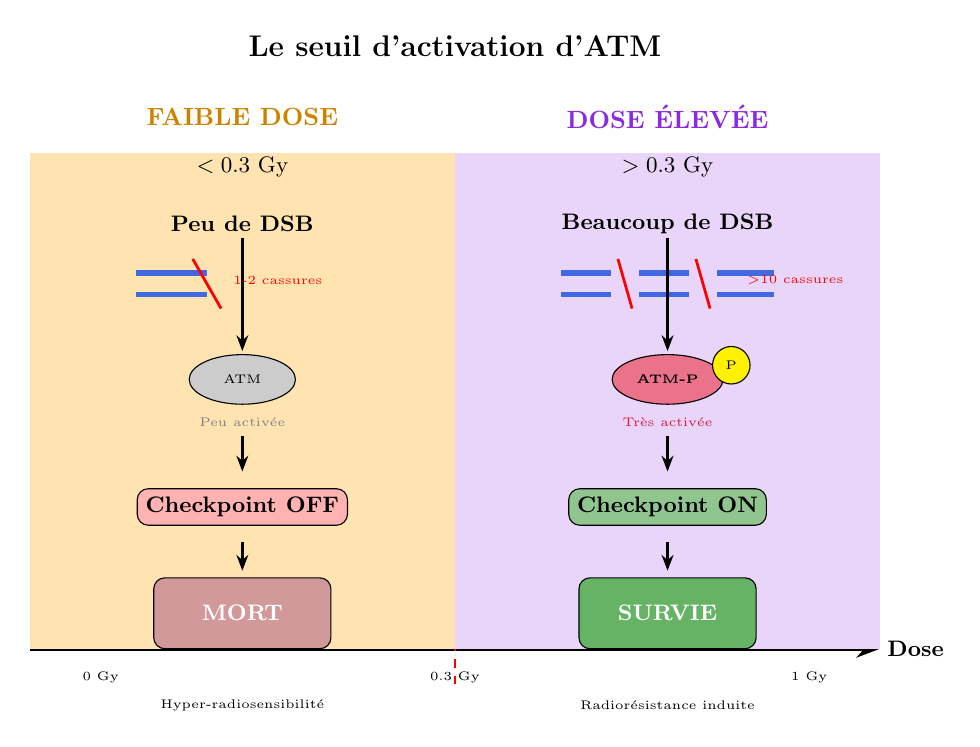
\begin{tikzpicture}[scale=0.9, transform shape]
    % Titre
    \node[font=\large\bfseries] at (0,8.5) {Le seuil d'activation d'ATM};
    
    % Axe des doses
    \draw[-{Stealth[length=3mm]}, line width=1.5pt] (-6,0) -- (6,0);
    \node[font=\small\bfseries] at (6.5,0) {Dose};
    \node[font=\tiny] at (-5,-0.4) {0 Gy};
    \node[font=\tiny] at (0,-0.4) {0.3 Gy};
    \node[font=\tiny] at (5,-0.4) {1 Gy};
    
    % Ligne de seuil
    \draw[dashed, line width=1pt, red] (0,-0.5) -- (0,7);
    \node[font=\small\bfseries, red, rotate=90] at (-0.5,3.5) {Seuil $D_c$};
    
    % Zone faible dose
    \fill[lowdose!30] (-6,0) rectangle (0,7);
    \node[font=\bfseries, lowdose!80!black] at (-3,7.5) {FAIBLE DOSE};
    \node[font=\small] at (-3,6.8) {$< 0.3$ Gy};
    
    % Zone dose plus élevée
    \fill[highdose!20] (0,0) rectangle (6,7);
    \node[font=\bfseries, highdose] at (3,7.5) {DOSE ÉLEVÉE};
    \node[font=\small] at (3,6.8) {$> 0.3$ Gy};
    
    % === Colonne gauche (faible dose) ===
    % Peu de DSB
    \node[font=\small\bfseries] at (-3,6) {Peu de DSB};
    \draw[dnacolor, line width=2pt] (-4.5,5.3) -- (-3.5,5.3);
    \draw[dnacolor, line width=2pt] (-4.5,5) -- (-3.5,5);
    \draw[red, line width=1pt] (-3.7,5.5) -- (-3.3,4.8);
    \node[font=\tiny, red] at (-2.5,5.2) {1-2 cassures};
    
    % ATM peu activée
    \node[draw, ellipse, fill=gray!40, minimum width=1.5cm, minimum height=0.7cm, font=\tiny] at (-3,3.8) {ATM};
    \node[font=\tiny, gray] at (-3,3.2) {Peu activée};
    
    % Checkpoint OFF
    \node[draw, rectangle, rounded corners, fill=red!30, minimum width=2cm, font=\small\bfseries] at (-3,2) {Checkpoint OFF};
    
    % Résultat
    \node[draw, rectangle, rounded corners, fill=deathcolor!40, minimum width=2.5cm, minimum height=1cm, font=\small\bfseries, text=white] at (-3,0.5) {MORT};
    \node[font=\tiny] at (-3,-0.8) {Hyper-radiosensibilité};
    
    % === Colonne droite (dose élevée) ===
    % Beaucoup de DSB
    \node[font=\small\bfseries] at (3,6) {Beaucoup de DSB};
    \draw[dnacolor, line width=2pt] (1.5,5.3) -- (2.2,5.3);
    \draw[dnacolor, line width=2pt] (2.6,5.3) -- (3.3,5.3);
    \draw[dnacolor, line width=2pt] (3.7,5.3) -- (4.5,5.3);
    \draw[dnacolor, line width=2pt] (1.5,5) -- (2.2,5);
    \draw[dnacolor, line width=2pt] (2.6,5) -- (3.3,5);
    \draw[dnacolor, line width=2pt] (3.7,5) -- (4.5,5);
    \draw[red, line width=1pt] (2.3,5.5) -- (2.5,4.8);
    \draw[red, line width=1pt] (3.4,5.5) -- (3.6,4.8);
    \node[font=\tiny, red] at (4.8,5.2) {$>$10 cassures};
    
    % ATM très activée
    \node[draw, ellipse, fill=atmcolor!60, minimum width=1.5cm, minimum height=0.7cm, font=\tiny\bfseries] at (3,3.8) {ATM-P};
    \node[draw, circle, fill=yellow, minimum size=0.3cm, font=\tiny] at (3.9,4) {P};
    \node[font=\tiny, atmcolor] at (3,3.2) {Très activée};
    
    % Checkpoint ON
    \node[draw, rectangle, rounded corners, fill=checkcolor!50, minimum width=2cm, font=\small\bfseries] at (3,2) {Checkpoint ON};
    
    % Résultat
    \node[draw, rectangle, rounded corners, fill=survivecolor!60, minimum width=2.5cm, minimum height=1cm, font=\small\bfseries, text=white] at (3,0.5) {SURVIE};
    \node[font=\tiny] at (3,-0.8) {Radiorésistance induite};
    
    % Flèches descendantes
    \draw[-{Stealth[length=2mm]}, line width=1pt] (-3,5.8) -- (-3,4.2);
    \draw[-{Stealth[length=2mm]}, line width=1pt] (-3,3) -- (-3,2.5);
    \draw[-{Stealth[length=2mm]}, line width=1pt] (-3,1.5) -- (-3,1.1);
    
    \draw[-{Stealth[length=2mm]}, line width=1pt] (3,5.8) -- (3,4.2);
    \draw[-{Stealth[length=2mm]}, line width=1pt] (3,3) -- (3,2.5);
    \draw[-{Stealth[length=2mm]}, line width=1pt] (3,1.5) -- (3,1.1);
\end{tikzpicture}
\caption{Comparaison de la réponse cellulaire aux faibles et fortes doses. Le seuil d'activation d'ATM ($D_c \approx 0.2-0.5$ Gy) détermine si le checkpoint sera activé ou non.}
\label{fig:seuil}
\end{figure}

\begin{table}[h!]
\centering
\caption{Comparaison des réponses cellulaires selon la dose}
\label{tab:comparaison}
\begin{tabular}{lcc}
\toprule
\textbf{Paramètre} & \textbf{Faible dose ($< D_c$)} & \textbf{Dose élevée ($> D_c$)} \\
\midrule
Nombre de DSB & Faible (1-5) & Élevé ($>$10) \\
Activation ATM & Faible/Absente & Forte \\
Checkpoint G2/M & Non activé & Activé \\
Devenir cellulaire & Mitose avec ADN cassé & Arrêt et réparation \\
\textbf{Résultat} & \textbf{MORT (HRS)} & \textbf{SURVIE (IRR)} \\
\bottomrule
\end{tabular}
\end{table}

\newpage
\section{Mécanisme détaillé de l'hyper-radiosensibilité}

\begin{figure}[h!]
\centering
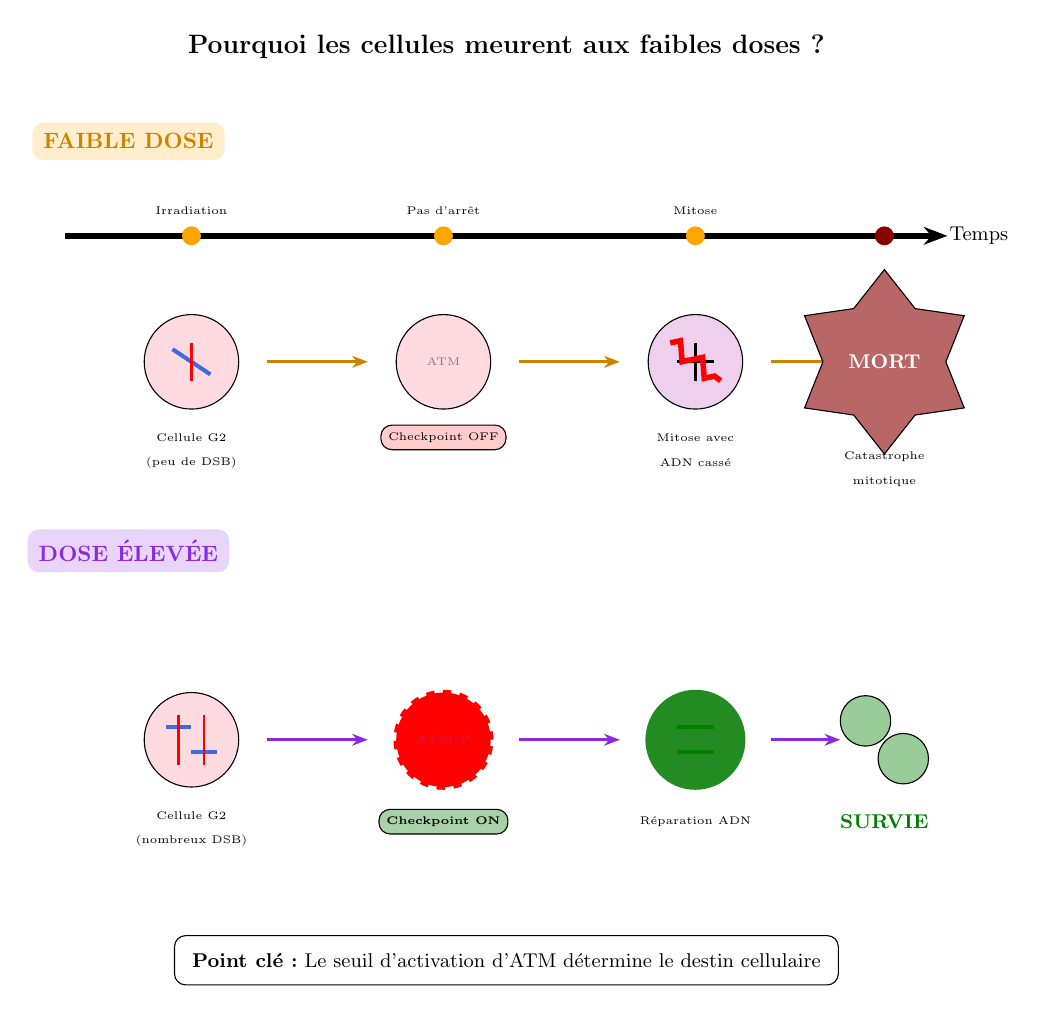
\begin{tikzpicture}[scale=0.8, transform shape]
    % Titre
    \node[font=\large\bfseries] at (0,10) {Pourquoi les cellules meurent aux faibles doses ?};
    
    % Timeline horizontale
    \draw[-{Stealth[length=3mm]}, line width=2pt] (-7,7) -- (7,7);
    \node[font=\small] at (7.5,7) {Temps};
    
    % === FAIBLE DOSE (haut) ===
    \node[font=\bfseries, lowdose!80!black, fill=lowdose!20, rounded corners, inner sep=5pt] at (-6,8.5) {FAIBLE DOSE};
    
    % Étape 1 : Cellule G2 irradiée
    \node[draw, circle, minimum size=1.5cm, fill=g2color!50] (c1) at (-5,5) {};
    \draw[dnacolor, line width=1.5pt] (-5.3,5.2) -- (-4.7,4.8);
    \draw[red, line width=1pt] (-5,5.3) -- (-5,4.7);
    \node[font=\tiny] at (-5,3.8) {Cellule G2};
    \node[font=\tiny] at (-5,3.4) {(peu de DSB)};
    
    % Point sur timeline
    \fill[lowdose] (-5,7) circle (0.15);
    \node[font=\tiny] at (-5,7.4) {Irradiation};
    
    % Flèche
    \draw[-{Stealth[length=2mm]}, line width=1pt, lowdose!80!black] (-3.8,5) -- (-2.2,5);
    
    % Étape 2 : ATM inactive, checkpoint non activé
    \node[draw, circle, minimum size=1.5cm, fill=g2color!50] (c2) at (-1,5) {};
    \node[font=\tiny, gray] at (-1,5) {ATM};
    \node[draw, rectangle, fill=red!20, font=\tiny, rounded corners] at (-1,3.8) {Checkpoint OFF};
    
    % Point sur timeline
    \fill[lowdose] (-1,7) circle (0.15);
    \node[font=\tiny] at (-1,7.4) {Pas d'arrêt};
    
    % Flèche
    \draw[-{Stealth[length=2mm]}, line width=1pt, lowdose!80!black] (0.2,5) -- (1.8,5);
    
    % Étape 3 : Entrée en mitose avec ADN cassé
    \node[draw, circle, minimum size=1.5cm, fill=mcolor!50] (c3) at (3,5) {};
    \draw[line width=1pt] (2.7,5) -- (3.3,5);
    \draw[line width=1pt] (3,4.7) -- (3,5.3);
    \draw[red, line width=2pt, decorate, decoration={zigzag, amplitude=1mm}] (2.6,5.3) -- (3.4,4.7);
    \node[font=\tiny] at (3,3.8) {Mitose avec};
    \node[font=\tiny] at (3,3.4) {ADN cassé};
    
    % Point sur timeline
    \fill[lowdose] (3,7) circle (0.15);
    \node[font=\tiny] at (3,7.4) {Mitose};
    
    % Flèche
    \draw[-{Stealth[length=2mm]}, line width=1pt, lowdose!80!black] (4.2,5) -- (5.3,5);
    
    % Étape 4 : Catastrophe mitotique / Mort
    \node[draw, star, star points=6, minimum size=1.8cm, fill=deathcolor!60, font=\small\bfseries, text=white] (death) at (6,5) {MORT};
    \node[font=\tiny] at (6,3.5) {Catastrophe};
    \node[font=\tiny] at (6,3.1) {mitotique};
    
    % Point sur timeline
    \fill[deathcolor] (6,7) circle (0.15);
    
    % === DOSE ÉLEVÉE (bas) ===
    \node[font=\bfseries, highdose, fill=highdose!20, rounded corners, inner sep=5pt] at (-6,2) {DOSE ÉLEVÉE};
    
    % Étape 1 : Cellule G2 irradiée
    \node[draw, circle, minimum size=1.5cm, fill=g2color!50] (c1b) at (-5,-1) {};
    \draw[dnacolor, line width=1.5pt] (-5.4,-0.8) -- (-5,-0.8);
    \draw[dnacolor, line width=1.5pt] (-5,-1.2) -- (-4.6,-1.2);
    \draw[red, line width=1pt] (-5.2,-0.6) -- (-5.2,-1.4);
    \draw[red, line width=1pt] (-4.8,-0.6) -- (-4.8,-1.4);
    \node[font=\tiny] at (-5,-2.2) {Cellule G2};
    \node[font=\tiny] at (-5,-2.6) {(nombreux DSB)};
    
    % Flèche
    \draw[-{Stealth[length=2mm]}, line width=1pt, highdose] (-3.8,-1) -- (-2.2,-1);
    
    % Étape 2 : ATM active, checkpoint activé
    \node[draw, circle, minimum size=1.5cm, fill=g2color!50, line width=2pt, dashed, red] (c2b) at (-1,-1) {};
    \node[font=\tiny\bfseries, atmcolor] at (-1,-1) {ATM-P};
    \node[draw, rectangle, fill=checkcolor!40, font=\tiny\bfseries, rounded corners] at (-1,-2.3) {Checkpoint ON};
    
    % Flèche
    \draw[-{Stealth[length=2mm]}, line width=1pt, highdose] (0.2,-1) -- (1.8,-1);
    
    % Étape 3 : Arrêt en G2, réparation
    \node[draw, circle, minimum size=1.5cm, fill=g2color!50, line width=2pt, checkcolor] (c3b) at (3,-1) {};
    \node[font=\tiny, checkcolor] at (3,-1) {ARRÊT};
    \draw[survivecolor, line width=1.5pt] (2.7,-0.8) -- (3.3,-0.8);
    \draw[survivecolor, line width=1.5pt] (2.7,-1.2) -- (3.3,-1.2);
    \node[font=\tiny] at (3,-2.3) {Réparation ADN};
    
    % Flèche
    \draw[-{Stealth[length=2mm]}, line width=1pt, highdose] (4.2,-1) -- (5.3,-1);
    
    % Étape 4 : Survie et division normale
    \node[draw, circle, minimum size=0.8cm, fill=survivecolor!40] at (5.7,-0.7) {};
    \node[draw, circle, minimum size=0.8cm, fill=survivecolor!40] at (6.3,-1.3) {};
    \node[font=\small\bfseries, survivecolor] at (6,-2.3) {SURVIE};
    
    % Légende
    \node[draw, rectangle, rounded corners, fill=white, inner sep=8pt, font=\small] at (0,-4.5) {
        \textbf{Point clé :} Le seuil d'activation d'ATM détermine le destin cellulaire
    };
\end{tikzpicture}
\caption{Comparaison des destins cellulaires aux faibles doses (haut, HRS) et aux doses plus élevées (bas, IRR). Le checkpoint G2/M non activé aux faibles doses conduit à la catastrophe mitotique.}
\label{fig:mecanisme}
\end{figure}

\newpage
\section{Analogie : le système d'alarme incendie}

Pour bien comprendre le phénomène, imaginons un \textbf{système d'alarme incendie} réglé pour ne se déclencher qu'à partir d'une certaine quantité de fumée.

\begin{figure}[h!]
\centering
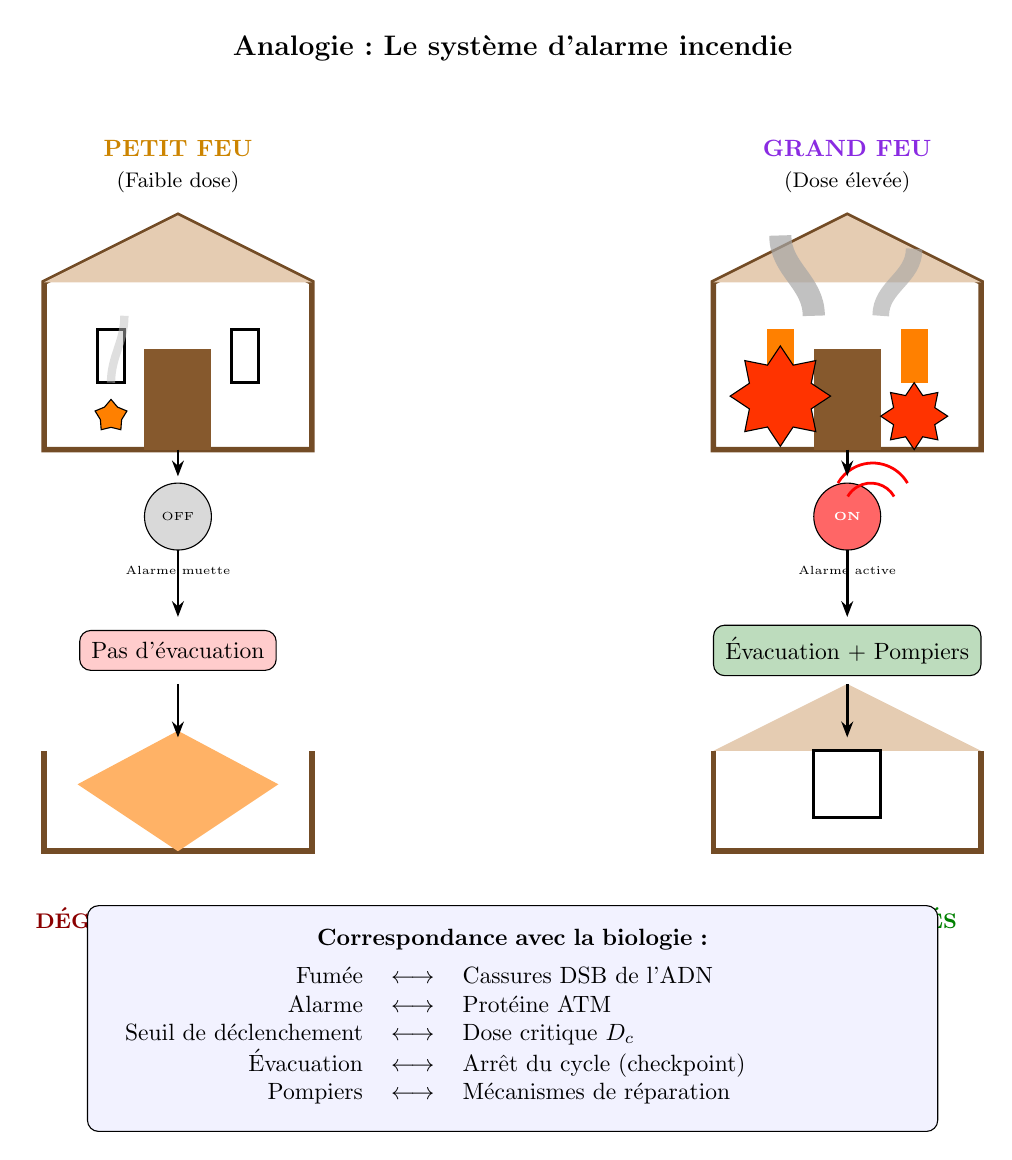
\begin{tikzpicture}[scale=0.85, transform shape]
    % Titre
    \node[font=\large\bfseries] at (0,9) {Analogie : Le système d'alarme incendie};
    
    % === PETIT FEU (gauche) ===
    \node[font=\bfseries, lowdose!80!black] at (-5,7.5) {PETIT FEU};
    \node[font=\small] at (-5,7) {(Faible dose)};
    
    % Maison avec petit feu
    \draw[line width=2pt, brown!60!black] (-7,3) -- (-7,5.5) -- (-5,6.5) -- (-3,5.5) -- (-3,3) -- cycle;
    \draw[line width=1.5pt, brown!60!black] (-7,3) -- (-3,3);
    % Toit
    \fill[brown!40] (-7,5.5) -- (-5,6.5) -- (-3,5.5) -- cycle;
    % Porte
    \fill[brown!70!black] (-5.5,3) rectangle (-4.5,4.5);
    % Fenêtre
    \draw[line width=1pt] (-6.2,4) rectangle (-5.8,4.8);
    \draw[line width=1pt] (-4.2,4) rectangle (-3.8,4.8);
    
    % Petit feu
    \node[draw, star, star points=5, fill=orange, minimum size=0.5cm] at (-6,3.5) {};
    % Peu de fumée
    \draw[gray!50, line width=3pt, opacity=0.5] (-6,4) to[out=90,in=-90] (-5.8,5);
    
    % Alarme silencieuse
    \node[draw, circle, minimum size=1cm, fill=gray!30] (alarm1) at (-5,2) {};
    \node[font=\tiny] at (-5,2) {OFF};
    \node[font=\tiny] at (-5,1.2) {Alarme muette};
    
    % Pas d'évacuation
    \node[draw, rectangle, rounded corners, fill=red!20, inner sep=5pt] at (-5,0) {Pas d'évacuation};
    
    % Résultat
    \draw[line width=2pt, brown!60!black] (-7,-1.5) -- (-7,-3) -- (-3,-3) -- (-3,-1.5);
    \fill[orange!60] (-6.5,-2) -- (-5,-1.2) -- (-3.5,-2) -- (-5,-3) -- cycle;
    \node[font=\small\bfseries, deathcolor] at (-5,-4) {DÉGÂTS IMPORTANTS};
    
    % Flèches
    \draw[-{Stealth[length=2mm]}, line width=1pt] (-5,3) -- (-5,2.6);
    \draw[-{Stealth[length=2mm]}, line width=1pt] (-5,1.5) -- (-5,0.5);
    \draw[-{Stealth[length=2mm]}, line width=1pt] (-5,-0.5) -- (-5,-1.3);
    
    % === GRAND FEU (droite) ===
    \node[font=\bfseries, highdose] at (5,7.5) {GRAND FEU};
    \node[font=\small] at (5,7) {(Dose élevée)};
    
    % Maison avec grand feu
    \draw[line width=2pt, brown!60!black] (3,3) -- (3,5.5) -- (5,6.5) -- (7,5.5) -- (7,3) -- cycle;
    \draw[line width=1.5pt, brown!60!black] (3,3) -- (7,3);
    % Toit
    \fill[brown!40] (3,5.5) -- (5,6.5) -- (7,5.5) -- cycle;
    % Porte
    \fill[brown!70!black] (4.5,3) rectangle (5.5,4.5);
    % Fenêtre avec flammes
    \fill[orange] (3.8,4) rectangle (4.2,4.8);
    \fill[orange] (5.8,4) rectangle (6.2,4.8);
    
    % Grand feu
    \node[draw, star, star points=8, fill=red!80!yellow, minimum size=1.5cm] at (4,3.8) {};
    \node[draw, star, star points=8, fill=red!80!yellow, minimum size=1cm] at (6,3.5) {};
    
    % Beaucoup de fumée
    \draw[gray!70, line width=8pt, opacity=0.7] (4.5,5) to[out=90,in=-90] (4,6.2);
    \draw[gray!70, line width=6pt, opacity=0.6] (5.5,5) to[out=90,in=-90] (6,6);
    
    % Alarme active
    \node[draw, circle, minimum size=1cm, fill=red!60] (alarm2) at (5,2) {};
    \node[font=\tiny\bfseries, white] at (5,2) {ON};
    \node[font=\tiny] at (5,1.2) {Alarme active};
    % Ondes sonores
    \draw[red, line width=1pt] (5.7,2.3) arc (30:150:0.4);
    \draw[red, line width=1pt] (5.9,2.5) arc (30:150:0.6);
    
    % Évacuation + Pompiers
    \node[draw, rectangle, rounded corners, fill=checkcolor!30, inner sep=5pt] at (5,0) {Évacuation + Pompiers};
    
    % Résultat
    \draw[line width=2pt, brown!60!black] (3,-1.5) -- (3,-3) -- (7,-3) -- (7,-1.5);
    \fill[brown!40] (3,-1.5) -- (5,-0.5) -- (7,-1.5) -- cycle;
    \draw[line width=1pt] (4.5,-1.5) rectangle (5.5,-2.5);
    \node[font=\small\bfseries, survivecolor] at (5,-4) {DÉGÂTS LIMITÉS};
    
    % Flèches
    \draw[-{Stealth[length=2mm]}, line width=1pt] (5,3) -- (5,2.6);
    \draw[-{Stealth[length=2mm]}, line width=1pt] (5,1.5) -- (5,0.5);
    \draw[-{Stealth[length=2mm]}, line width=1pt] (5,-0.5) -- (5,-1.3);
    
    % Correspondance
    \node[draw, rectangle, rounded corners, fill=blue!5, inner sep=10pt, text width=12cm] at (0,-5.5) {
        \centering
        \textbf{Correspondance avec la biologie :}\\[5pt]
        \begin{tabular}{rcl}
        Fumée & $\longleftrightarrow$ & Cassures DSB de l'ADN \\
        Alarme & $\longleftrightarrow$ & Protéine ATM \\
        Seuil de déclenchement & $\longleftrightarrow$ & Dose critique $D_c$ \\
        Évacuation & $\longleftrightarrow$ & Arrêt du cycle (checkpoint) \\
        Pompiers & $\longleftrightarrow$ & Mécanismes de réparation
        \end{tabular}
    };
\end{tikzpicture}
\caption{Analogie entre le système d'alarme incendie et le checkpoint G2/M. Le seuil de déclenchement de l'alarme correspond à la dose critique $D_c$ d'activation d'ATM.}
\label{fig:analogie}
\end{figure}

\newpage
\section{Schéma récapitulatif}

\begin{figure}[h!]
\centering
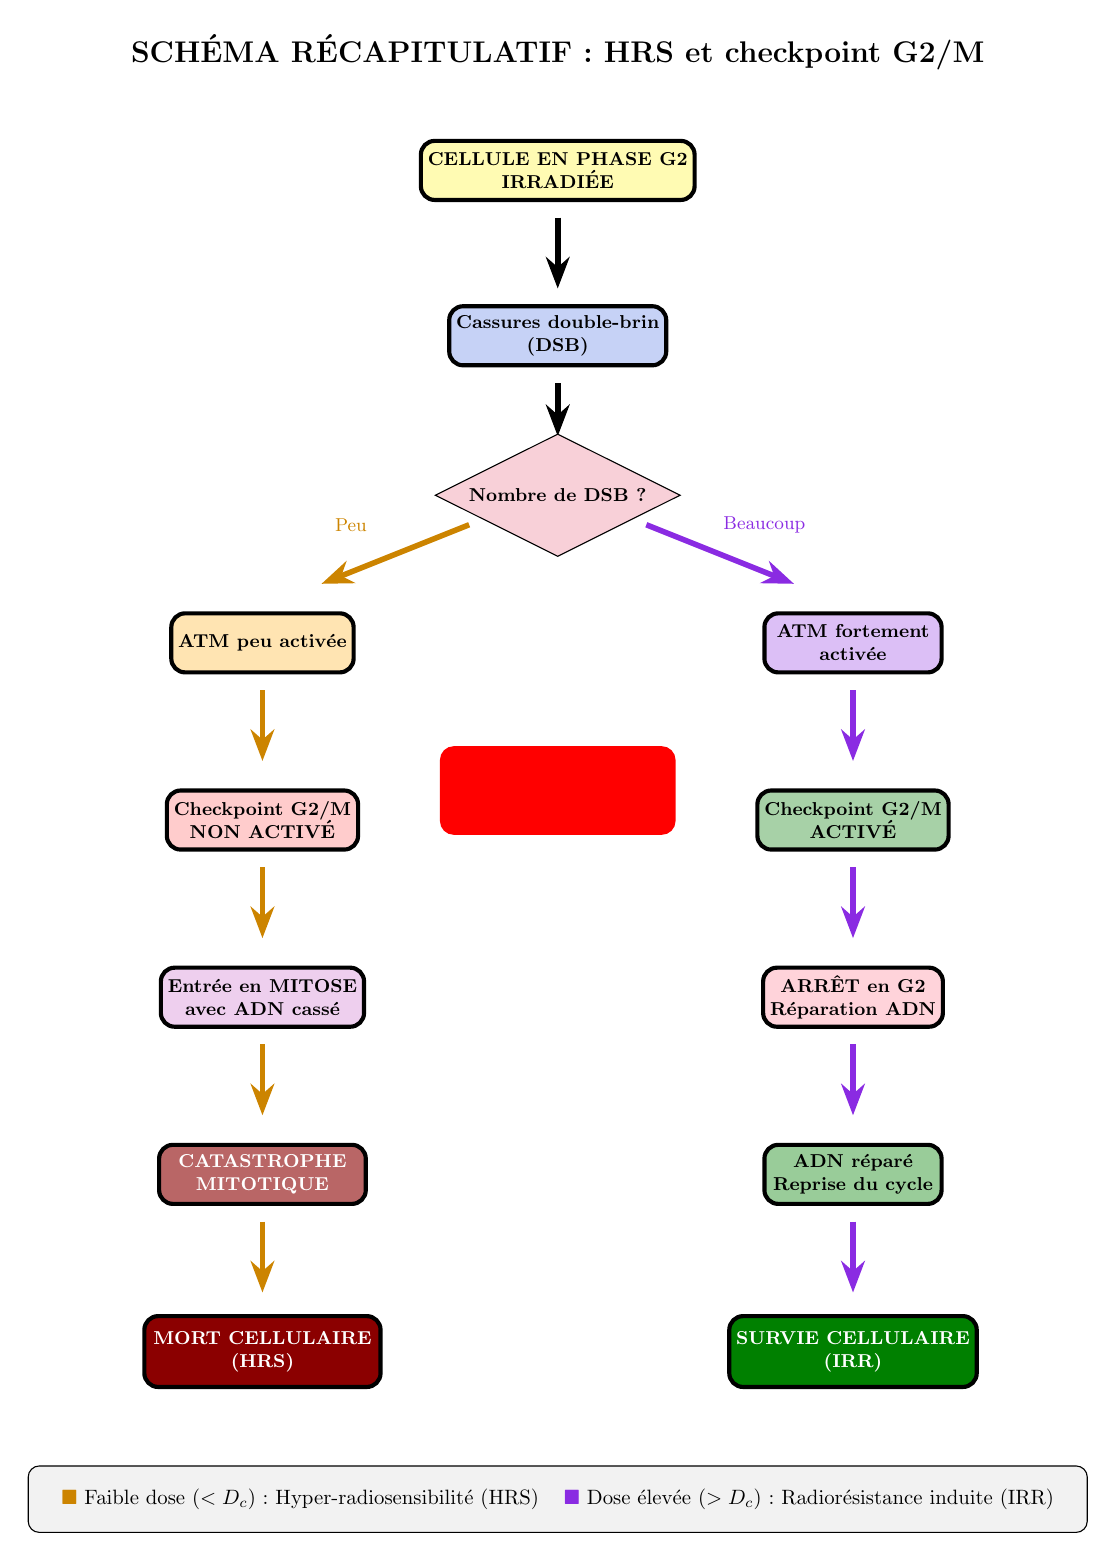
\begin{tikzpicture}[
    scale=0.75, 
    transform shape,
    box/.style={draw, rectangle, rounded corners=5pt, minimum width=3cm, minimum height=1cm, font=\small\bfseries, line width=1.5pt, align=center},
    arrow/.style={-{Stealth[length=4mm]}, line width=2pt}
]
    % Titre
    \node[font=\Large\bfseries] at (0,12) {SCHÉMA RÉCAPITULATIF : HRS et checkpoint G2/M};
    
    % Point de départ
    \node[box, fill=yellow!30, minimum width=4cm] (start) at (0,10) {CELLULE EN PHASE G2\\IRRADIÉE};
    
    % Branche
    \draw[arrow] (0,9.2) -- (0,8);
    \node[box, fill=dnacolor!30] (dsb) at (0,7.2) {Cassures double-brin\\(DSB)};
    
    % Division
    \draw[arrow] (0,6.4) -- (0,5.5);
    \node[draw, diamond, aspect=2, fill=atmcolor!20, minimum width=3cm, font=\small\bfseries] (decision) at (0,4.5) {Nombre de DSB ?};
    
    % === Branche GAUCHE (faible dose) ===
    \draw[arrow, lowdose!80!black] (-1.5,4) -- (-4,3);
    \node[font=\small, lowdose!80!black] at (-3.5,4) {Peu};
    
    \node[box, fill=lowdose!30] (low1) at (-5,2) {ATM peu activée};
    \draw[arrow, lowdose!80!black] (-5,1.2) -- (-5,0);
    
    \node[box, fill=red!20] (low2) at (-5,-1) {Checkpoint G2/M\\NON ACTIVÉ};
    \draw[arrow, lowdose!80!black] (-5,-1.8) -- (-5,-3);
    
    \node[box, fill=mcolor!50] (low3) at (-5,-4) {Entrée en MITOSE\\avec ADN cassé};
    \draw[arrow, lowdose!80!black] (-5,-4.8) -- (-5,-6);
    
    \node[box, fill=deathcolor!60, text=white, minimum width=3.5cm] (low4) at (-5,-7) {CATASTROPHE\\MITOTIQUE};
    \draw[arrow, lowdose!80!black] (-5,-7.8) -- (-5,-9);
    
    \node[box, fill=deathcolor, text=white, minimum width=4cm, minimum height=1.2cm] (death) at (-5,-10) {MORT CELLULAIRE\\(HRS)};
    
    % === Branche DROITE (dose élevée) ===
    \draw[arrow, highdose] (1.5,4) -- (4,3);
    \node[font=\small, highdose] at (3.5,4) {Beaucoup};
    
    \node[box, fill=highdose!30] (high1) at (5,2) {ATM fortement\\activée};
    \draw[arrow, highdose] (5,1.2) -- (5,0);
    
    \node[box, fill=checkcolor!40] (high2) at (5,-1) {Checkpoint G2/M\\ACTIVÉ};
    \draw[arrow, highdose] (5,-1.8) -- (5,-3);
    
    \node[box, fill=g2color!60] (high3) at (5,-4) {ARRÊT en G2\\Réparation ADN};
    \draw[arrow, highdose] (5,-4.8) -- (5,-6);
    
    \node[box, fill=survivecolor!40] (high4) at (5,-7) {ADN réparé\\Reprise du cycle};
    \draw[arrow, highdose] (5,-7.8) -- (5,-9);
    
    \node[box, fill=survivecolor, text=white, minimum width=4cm, minimum height=1.2cm] (survive) at (5,-10) {SURVIE CELLULAIRE\\(IRR)};
    
    % Encadré dose critique
    \node[draw, rectangle, rounded corners, fill=white, inner sep=8pt, line width=2pt, red] at (0,-0.5) {
        \begin{tabular}{c}
        \textbf{Dose critique $D_c$}\\
        $\approx 0.2 - 0.5$ Gy
        \end{tabular}
    };
    
    % Légende
    \node[draw, rectangle, rounded corners, fill=gray!10, inner sep=10pt] at (0,-12.5) {
        \begin{tabular}{ll}
        \textcolor{lowdose!80!black}{$\blacksquare$} Faible dose ($< D_c$) : Hyper-radiosensibilité (HRS) &
        \textcolor{highdose}{$\blacksquare$} Dose élevée ($> D_c$) : Radiorésistance induite (IRR)
        \end{tabular}
    };
\end{tikzpicture}
\caption{Schéma récapitulatif du rôle du checkpoint G2/M dépendant d'ATM dans le phénomène d'hyper-radiosensibilité. La dose critique $D_c$ détermine si le checkpoint est activé ou non.}
\label{fig:recap}
\end{figure}

\newpage
\section{Conclusion}

Le checkpoint G2/M dépendant d'ATM joue un rôle central dans le phénomène d'hyper-radiosensibilité aux faibles doses :

\begin{enumerate}
    \item \textbf{ATM agit comme un senseur} des dommages à l'ADN, mais nécessite un seuil minimum de cassures pour s'activer efficacement.
    
    \item \textbf{Aux faibles doses} ($< D_c \approx 0.2-0.5$ Gy), le nombre de cassures est insuffisant pour activer pleinement ATM et le checkpoint G2/M.
    
    \item \textbf{Sans arrêt du cycle}, les cellules endommagées entrent en mitose avec des cassures non réparées, conduisant à la catastrophe mitotique et à la mort cellulaire.
    
    \item \textbf{Aux doses plus élevées}, ATM est activée, le checkpoint bloque les cellules en G2, permettant la réparation de l'ADN avant la mitose.
    
    \item Ce mécanisme explique le \textbf{paradoxe apparent} où les cellules survivent mieux à des doses modérées qu'à de très faibles doses.
\end{enumerate}

\vspace{1cm}

\begin{thebibliography}{99}

\bibitem{Marples2004}
Marples B, Wouters BG, Collis SJ, Chalmers AJ, Joiner MC.
\textit{Low-dose hyper-radiosensitivity: a consequence of ineffective cell cycle arrest of radiation-damaged G2-phase cells.}
Radiat Res. 2004;161(3):247-255.

\bibitem{Krueger2010}
Krueger SA, Wilson GD, Piasentin E, Joiner MC, Marples B.
\textit{The effects of G2-phase enrichment and checkpoint abrogation on low-dose hyper-radiosensitivity.}
Int J Radiat Oncol Biol Phys. 2010;77(5):1509-1517.

\bibitem{Fernet2010}
Fernet M, Mégnin-Chanet F, Hall J, Favaudon V.
\textit{Control of the G2/M checkpoints after exposure to low doses of ionising radiation: implications for hyper-radiosensitivity.}
DNA Repair. 2010;9(1):48-57.

\bibitem{Bakkenist2003}
Bakkenist CJ, Kastan MB.
\textit{DNA damage activates ATM through intermolecular autophosphorylation and dimer dissociation.}
Nature. 2003;421(6922):499-506.

\bibitem{Xu2002}
Xu B, Kim ST, Lim DS, Kastan MB.
\textit{Two molecularly distinct G2/M checkpoints are induced by ionizing irradiation.}
Mol Cell Biol. 2002;22(4):1049-1059.

\end{thebibliography}

\end{document}
